\chapter{Extend's Internal Architecture}

\begin{center}
  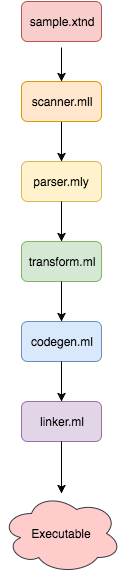
\includegraphics[width=.20\textwidth, height=15cm]{img/Execution.png}
\end{center}

\newpage

\section{The Extend Compiler}
The Extend compilation process consists of several source files, each of which performs a different function in the compilation pipeline.

\begin{itemize}
  \item \texttt{scanner.mll}: OCamllex scanner - consumes tokens.
  \item \texttt{parser.mly}: OCamlyacc parser - represents the Extend grammar.
  \item \texttt{ast.ml}: Abstract Syntax Tree, created from the output of the parser and representing the structure of an Extend program.
  \item \texttt{transform.ml}: Performs syntactic desugaring for easier compilation.
  \item \texttt{semant.ml}: Analyzes the semantics of the program to ensure that the program adheres to the rules of the language.
  \item \texttt{codegen.ml}: The LLVM IR code generator.
  \item \texttt{linker.ml}: Calls intermediary compilation steps on the generated \texttt{.ll}, including external functions if needed.
\end{itemize}

  \subsection{The Scanner}
  The function of \texttt{scanner.mll} is to parse a text stream into various tokens to be used in an Extend program.
  Only the tokens that are valid in Extend are to be given to the parser; all others will return a syntax error marked by the line and character number.

  \subsection{The Parser and Abstract Syntax Tree}
  The parser converts the tokens read by the scanner into a syntax tree deemed acceptable grammar within the Extend Language. This is converted into an Abstract Syntax Tree, which has nodes that can be consumed by the back end of the Extend compiler.

  \subsection{The Transformer}
The transformer is the first step in converting the AST into LLVM code. It takes the AST and reduces its breadth. This step is done to preserve the convenience for the user, but reduces the complexity for the actual compile step. A large number of internal variables are created in the process.

  \medskip \noindent This is how the user declares a variable.
  \begin{lstlisting}
    [2,2] foo;
  \end{lstlisting}

  \medskip \noindent This is how the transformer desugars the same code.
  \begin{lstlisting}
    rows_of_foo := 2;
    cols_of_foo := 2;
    [rows_of_foo, cols_of_foo] foo;
  \end{lstlisting}

  \medskip \noindent
  A similar transformation is performed on formula assignments:
  \begin{lstlisting}
    // Before Transformation:
    foo[g(x):4,3+3] = "Couldn't you have stuck to integers?";

    // After Transformation:
    start_row := g(x);
    end_row   := 4;
    start_col := 3+3;
    foo[start_row:end_row,start_col] = "Couldn't you have stuck to integers?";
  \end{lstlisting}
  \medskip \noindent
  Every expression on the left hand side before or after a comma or colon will become an internal temporary variable in the desugaring process. Internal variables are also created for the return expression and for any size assertions induced by the function signature:
  \begin{lstlisting}
    // Before Transformation:
    foo([m,n] arg1, [m, 1] arg2) {
      return m*n;
    }

    // After Transformation:
    foo(arg1, arg2) {
      m := numRows(arg1);
      n := numCols(arg1);
      asserts := (m == numRows(arg2)) && (1 == numCols(arg2));
      return_value := m*n;
      return return_value;
    }
  \end{lstlisting}
  In addition to generating temporary variables, Extend also transforms \texttt{\&\&, ||, and switch} into ternary conditionals to enable short-circuiting. Finally, the transformer performs some semantic analysis to ensure that there are no duplicate variables within a function, and no duplicate functions within a program.

  \subsection{The Semantic Analyzer}
  The semantic analyzer consumes the reduced AST. It ensures that Extend functions, variables, expressions, and more are being used properly at compile time, and throws flavorful exceptions to the user so that they may better understand why their program was illegal. In Extend, there are no real type errors involving expressions on the right-hand-side of a formula, as we attempt to degrade many gracefully. There are type errors possible on the left-hand side, but since they are assigned dynamically, very few can be determined at compile time. For function calls, the semantic analyzer ensures that the function exists and is called with the right number of arguments; and for variables, the analysis checks that the identifier refers to a real variables within the appropriate scope.

  \subsection{The Code Generator}
 Once the Extend AST passes semantic analysis, the code generator turns the reduced AST into LLVM code. Since the variable evaluation approach of Extend is not imperative, this process is fairly elaborate. There is one function created per formula, which is available to be called if the value of a cell with that formula is needed; and there is one function created per Extend function, which initializes a scope object with a collection of blueprints for all the local variables of that function. In its most basic form, each blueprint has a reference to one or more formulas that calculate the value of the variable. The section on the runtime goes into more detail on how this architecture is used.

  \subsection{The Linker}
  If successful LLVM IR is generated, the linker will adopt the role of building an executable object from the \texttt{.ll} file. This includes compiling it to an object file and linking the runtime environment along with other imported libraries.

  \section{Extend Runtime}
  Extend's cell values are lazily evaluated, which means they need to be implemented using function pointers. For each function that the Extend developer writes, the corresponding LLVM function that is generated is essentially identical: allocate a scope object for that function call, initialize that object with the appropriate set of variable definitions and the function arguments to that scope object, and then evaluate the variables corresponding to the size assertion and the return expression for that function. All of the "individualized" code lives in what we refer to as the formula-functions; for each distinct formula, the compiler generates a corresponding function that can be called when the corresponding cell's value is needed. Each formula-function shares the same signature: the arguments are a pointer to a scope and the row and column number of the cell being evaluated, and the return value is a pointer to a value struct (which holds the type and contents of the value.)

  The two main functions of our C runtime, therefore, are instantiate\_variable(), which looks at the variable definition "blueprint" and calculates the actual dimensions of the variable for that particular function call, and calculates the actual range of cells to which each formula applies; and getVal(), which determines if a particular cell value has already been calculated or not, and calls the appropriate formula-function if not.

  Before actually calling the main Extend entry point, our executable initializes a global array with the appropriate variable definitions for each function. When an Extend function is called, it simply copies the appropriate pointer into that array into its scope object.

  Leaving aside the variables introduced by the transformation step, this Extend function:
  \begin{lstlisting}
    foo() {
      x := 1;
      return x;
    }
  \end{lstlisting}
  \medskip \noindent
  would result in the LLVM equivalent of the following pseudocode (not written in any actual language) being generated:

  \begin{lstlisting}
    value_p foo() {
      scope = new ExtendScope;

      // Load the apropriate set of definitions for foo
      scope->defns = global_definitions[42];

      // Create an array of pointers to variable instances; one
      // pointer per variable. Only one variable in this function
      scope->insts = new var_instance* [1];

      // getVar calls instantiate_var if that instance pointer is still NULL,
      // or just returns the pointer if it's already been instantiated.
      // The instantiated variable keeps a copy of the pointer to its scope
      var_instance *return_variable = getVar(scope, 0);

      // Get the value of cell [0,0] of return_variable
      return getVal(return_variable, 0, 0);
    }
  \end{lstlisting}
  \medskip \noindent

  Since the newly initialized scope object will hold all NULL pointers for the instances, getVar() will end up calling instantiate\_variable, which will  determine that x has 1 row and 1 column; there is only a single formula for x, applying to all cells of x; and that that formula corresponds to the function pointer indicated in the variable definition.
  When getVal is called, the value pointer for the [0,0]th cell will similarly be NULL. As a result, getVal() will determine the function pointer for the appropriate formula and then call it, supplying as arguments a pointer to the scope and (0,0) for the row and column.

  The actual C structures used are listed below:
  \begin{lstlisting}

  // Each formula-function has the following signature:
  typedef value_p (*FormulaFP) (struct ExtendScope *scope, int row, int col);

  // This structure tells the runtime how to actually calculate the range of
  // cells to which each formula applies.
  struct ExtendFormula {
    /* These 10 variables correspond to formula_row_start through formula_col_end,
     * where char singleRow/Col are true if formula_row_end is None */
    char fromFirstRow;
    int rowStart_varnum;
    char toLastRow;
    int rowEnd_varnum;
    char fromFirstCol;
    int colStart_varnum;
    char toLastCol;
    int colEnd_varnum;

  	char isSingleRow;
  	char isSingleCol;

    FormulaFP formula;
  };

  // For a particular variable instance, this structure holds the results
  // of the calculations for each formula.
  struct ResolvedFormula {
  	int rowStart, rowEnd, colStart, colEnd;
  	FormulaFP formula;
  };

  struct var_defn {
    /* This is like a class definition - for every declared variable in the
     * Extend source, there should be one instance of these per compiled program.
     * They should just live in the global program storage.
     * It corresponds to Ast.variable */
     int rows_varnum;
     int cols_varnum;
     int numFormulas;
     struct ExtendFormula *formulas;
  	 char isOneByOne;
  	 char *name;
  };

  struct var_instance {
    /* This is an actual instance of a variable - we get one of these
     * per variable per time a function is called (assuming the contents
     * of the variable get examined.  */
  	int rows, cols;
  	int numFormulas;
  	struct ResolvedFormula *formulas;
    struct ExtendScope *closure;
    value_p *values;
  	char *status;
  	char *name;
  };

  // One scope object gets created per Extend function call
  struct ExtendScope {
    struct var_defn *defns;
    struct var_instance **vars;
  	int numVars;
  	int refcount;
  	value_p *functionParams;
  };
  \end{lstlisting}
